%\usepackage{listings}
%\usepackage{xcolor}   % optional, for nicer colours

%\lstset{
%  basicstyle=\small\ttfamily,
%  keywordstyle=\color{blue},
%  commentstyle=\color{gray},
%  stringstyle=\color{orange},
%  showstringspaces=false,
%  breaklines=true,
%  frame=single,
%  numbers=left,
%  numberstyle=\tiny,
%  tabsize=4
%}

\chapter{QPU Abstraction Framework for benchmarking}
\label{chap:QPU-framework-CEA-LIST}

This chapter describes the core object-oriented architecture used throughout the Benchmarking framework and its libraries.  
The design centres on a single abstract base class that acts as a uniform canvas for every QPU implementation.  Concrete QPU classes are realised by derivation, while a capability dictionary provides a completely target-independent call interface to the main program.  Generic (QPU-independent) computational kernels live in dedicated library modules; only the truly platform-specific fragments reside inside the concrete QPU modules.

The presentation is deliberately dual-audience: UML-aware readers will recognise the classic Abstract-Base-Class / Template-Method pattern; readers unfamiliar with UML can simply follow the textual explanations and the accompanying diagrams.

The CPU hardware provides a compatible class that implements reference CPU algorithms and heuristics. This is particularly important to provide reference scores to compare classic computing and quantum computing.

\section{Overall Architecture}

\begin{center}
\begin{tikzpicture}[
  class/.style={
    rectangle, draw, rounded corners=2pt,
    minimum width=3.8cm, minimum height=1.1cm,
    align=center, font=\small\ttfamily
  },
  abstract/.style={class, fill=blue!8},
  concrete/.style={class, fill=green!10},
  context/.style={class, fill=orange!12},
  arrow/.style={-stealth, thick},
  note/.style={font=\footnotesize\itshape, text width=3.2cm, align=left}
]
  % Abstract base
  \node[abstract] (base) at (-4.2,3.5)
    {BaseAbstractClass\\[-1pt]
     \footnotesize (ABC)};

  % Abstract base
  \node[abstract] (qpubase) at (0,3.5)
    {QPUBenchClass\\[-1pt]
     \footnotesize (ABC)};

  % Context
  \node[context] (ctx) at (04.2,3.5)
    {QPUContext\\[-1pt]
     \footnotesize (dataclass)};

  % Concrete QPUs
  \node[concrete] (qpu1) at (-4.2,0.8)
    {MyQPUA\\[-1pt]
     \footnotesize (Dwave)};
  \node[concrete] (qpu2) at (0,0.8)
    {MyQPUB\\[-1pt]
     \footnotesize (Pasqal)};
  \node[concrete] (qpu3) at (4.2,0.8)
    {MyQPUC\\[-1pt]
     \footnotesize (CPU)};

  % Inheritance arrows
  \draw[arrow] (qpubase) -- (base);
  \draw[arrow] (qpu1) -- (qpubase);
  \draw[arrow] (qpu2) -- (qpubase);
  \draw[arrow] (qpu3) -- (qpubase);

  % Usage
  \draw[arrow, dashed] (qpubase) -- node[below=5mm of qpubase, pos=3, font=\footnotesize] {uses / may inherit} (ctx);

  % Notes
  \node[note, anchor=west] at (-1.5,4.8)
    {Defines the contract\\
     (abstract methods +\\
     \texttt{capabilitySet})};
  \node[note, anchor=west] at (-6.0,1.8)
    {Must implement every\\
     abstract method};
\end{tikzpicture}
\end{center}

\begin{itemize}
  \item \textbf{QPUBenchClass} -- the single canvas every QPU must respect.
  \item \textbf{Concrete classes} (\texttt{MyQPU\_A}, \texttt{MyQPU\_B}, \ldots) -- one class per supported hardware target. The framework also provides a CPU backend for comparison between classical computing and quantum computing.
  \item \textbf{QPUContext} -- a lightweight data container (Python \texttt{@dataclass}) that carries all values and intermediate structures between the generic framework and the QPU-specific code.  Concrete QPUs may use it directly or derive a specialised context from it.
\end{itemize}

\section{BaseAbstractClass}

The abstract base class declares the mandatory interface and owns the central \texttt{capabilitySet} dictionary.

\subsection{Base principle and implementation}

\begin{lstlisting}[language=Python, caption={Definition of QPUContext and BaseAbstractClass}]
from abc import ABC, abstractmethod
from dataclasses import dataclass
from typing import Dict, Callable, Any
import argparse

@dataclass
class QPUContext:
    """Carrier of all data exchanged between
       generic framework code and QPU-
       specific implementations."""
    # common fields (arrays, scalars, handles ...)
    ...

class QPUBenchClass(ABC):
	@property
	# In the property part, derived (concrete) classes must define:
	# - capabilitySet -> list of strings: is the set of benchmark scores supported by the derived class 
	# - qpuDispatch -> dictionnary of list of function pointers. The key is the name of the benchmark that must be in the capabilitySet list 
	# - a QPUcontext to exchange the relevant data between functions and to the frontend 
	# - 3 function pointers preprocessMethod, computeMethod and postprocessMethod to call the relevant functions according to the bencmark score to run 
	
	@abstractmethod
	def capabilities(self) -> QPUBenchClassCapability:
		pass
        
	@abstractmethod
	def selectBenchmark(self, bench: str, **kwargs):
		# generic method to set the function pointers self.preprocessMethod, self.computeMethod and self.postprocessMethod 
		# the class methods below will make the actual call. The function pointers are allocated according to the selected benchmark 
		# it is worth noting that selectBenchmark method is (ATM) aimed to be called at the instatiation (by the constructor)
		pass

	@abstractmethod
	def preprocess(self, data: Any, **kwargs) -> Any:
		# method to call the self.preprocessMethod with the context
		pass

	@abstractmethod
	def compute(self, data: Any, **kwargs) -> Any:
		# method to call the self.computeMethod with the context
		pass

	@abstractmethod
	def postprocess(self, data: Any, **kwargs) -> Any:
		# method to call the self.postprocessMethod with the context
		pass

	@abstractmethod
	def is_available(self) -> bool:
		r"""Check if the QPU is available at runtime."""
		pass        

	@classmethod
	def add_arguments(cls, parser:argparse.ArgumentParser):
		r"""Generic class method to add arguments to the cli invocation depending on instancied class. """
      	"""Extend the global CLI with target-specific options (device id, layout, architecture, ...)."""
        pass

    # The three methods below are the concrete realisations
    # of the three entries in capabilitySet.  They are still
    # declared abstract so that every derived class is forced
    # to supply an implementation.
    @abstractmethod
    def preprocess(self, ctx: QPUContext) -> None:
        """Prepare the QPU and set its context."""
        ...

    @abstractmethod
    def run(self, ctx: QPUContext) -> None:
        """Execute the computation on the QPU."""
        ...

    @abstractmethod
    def postprocess(self, ctx: QPUContext) -> Any:
        """Post-process the result and return a
           target-independent set of results."""
        ...
\end{lstlisting}



\subsection{The \texttt{capabilitySet} list}

\texttt{capabilitySet} is a list of strings that provides all the benchmark scores currently supported by the concrete instance of QPUBenchClass.
The benchmark names must be constistent for all the QPU and all the instances. 
The names of the benchmarks also provide the key to look in the dictionnary of function pointers \texttt{qpuDispatch} as described below.

\subsection{The \texttt{qpuDispatch} dictionary}

The dictionary \texttt{capabilitySet} is the sole communication channel used by the main program.  It always contains exactly three function pointers:

\begin{center}
\begin{tabular}{|l|p{9.5cm}|}
\hline
\textbf{Key} & \textbf{Responsibility} \\
\hline
\texttt{"preprocess"}  & Prepare the QPU (allocate buffers, transfer data, configure the device, \ldots) and finalise the \texttt{QPUContext}. \\
\hline
\texttt{"compute"}         & Perform the actual computation on the QPU. \\
\hline
\texttt{"postprocess"} & Retrieve results from the device, free resources and return a completely target-independent set of results. \\
\hline
\end{tabular}
\end{center}

The main program never calls an QPU method by name.  It only calls the generic methods that, in turn, invokes the corresponding function pointer:

\begin{lstlisting}[language=Python]
		qpu.preprocess()
		qpu.compute()
		benchdone, score= qpu.postprocess()
\end{lstlisting}

This keeps the whole framework completely independent of any particular QPU.


\section{QPUBenchContext}

The data-class QPUBenchClass is the main communication means between the concrete instance of a QPUBenchClass to support a given QPU on one hand and on the other hand, both the specific functions implementing e.g. Register allocation on the QPU (or setting the stage for the computation) and also the main program implemented from \texttt{BACQBenchmak.py}.
The important aspects for this data class are:
\begin{itemize}
	\item \texttt{nIter}: which provides the current interation of the current benchmark executing on the QPU. Note that this is the responsability of \texttt{BACQBenchmak} to increment this counter.
	\item \texttt{dat}: an optional secondary value to perform the given benchmark (e.g. number of run for each iteration). The responsability of this variable depends usually on the particular benchmark.
	\item \texttt{currentBench}: String value giving the normalized name of the benchmark within the program (the same which is used to look in the dictionnary of the class) (\texttt{BACQBenchmak}). It serves in order to attribute the correct function pointers in the dictionnary.
	\item \texttt{formatedSamples}: are the samples returned by the QPU after run. They maybe QPU dependent, but should serve as a base to communicate the results to the postprocess method. N.B.: the postprocess method return QPU independent formated samples.
\end{itemize}

For all practical purposes, it is possible to inherit this class to implement more relevant context management for a given QPU, but any inherited class should provide the same base as the generic class with the same semantic for the common parts.

%%%
\section{Concrete QPU Classes}\label{sec:concreteQPU}

This section provides the principles of implementation of a QPU class inherited from \texttt{QPUBenchClass} to provide seamless support and inclusion into the multi-QPU benchmarking framework.

\subsection{Implementation contract}

Every concrete QPU class must:

\begin{enumerate}
  \item inherit from \texttt{BaseQPUClass},
  \item implement \emph{all} abstract methods (including \texttt{add\_argument}, \texttt{preprocess}, \texttt{run} and \texttt{postprocess}),
  \item bind the three life-cycle methods to the corresponding entries of \texttt{self.capabilitySet}.
\end{enumerate}

QPU-specific helper functions that are not part of the public contract live in the same Python module, usually at the top of the file, outside the class body.  Purely generic kernels (e.g.\ QUBO problem generation that does not depend specificly on the target) are placed in a separate computation library module and are imported by every concrete QPU that needs them.

\subsection{Typical file layout for one QPU}

Therefore, adding a new QPU to the set of supported QPU only consists in creating a concrete instance derivated from QPUBenchClass, on one hand, and adding the entries in the backend dictionary in the \texttt{BACQBenchmak.py} main program in the python dictionary \texttt{backendMap}.

Below, the base principle to implement a concrete QPU class.

\begin{lstlisting}[language=Python, caption={Example of a concrete QPU module}]
# my_QPU_shiny.py

# ------------------------------------------------------------------
# 1. QPU-specific low-level helpers
# ------------------------------------------------------------------
def _qpu_register_alloc(...): ...
def _qpu_sample_read(...): ...
def _qpu_launch_kernel(...): ...

# ------------------------------------------------------------------
# 2. Concrete class
# ------------------------------------------------------------------
class MyQPU1(QPUBenchClass):
    capabilitySet= ['gscore', ...] # capabilitySet is required to support at least one benchmark score 
    qpuDispatch= {'gscore':[qpuPreprocessGScore, qpuCompute, qpuPostprocessGScore], ...} # the dictionnary with the relevant function pointers
    QPUContext ctx
    
    def __init__(self, bench):
        super().__init__()
        # Bind the three mandatory capabilities (qpuDispatch is the dictionnary for the function pointers)
        selectBenchmark(bench)
    
    def selectBenchmark(self, bench: str, **kwargs):
        processSet= self.qpuDispatch[bench]
        self.myPreprocess= processSet[0]
        self.myCompute= processSet[1]
        self.myPostprocess= processSet[2]

    def add_argument(self, parser):
        parser.add_argument("--qpu1-device", type=sting, default='defaultarch')
        parser.add_argument("--qpu1-alg-select", ...)
        ...

    def preprocess(self, ctx: QPUContext):
        # allocate, copy host->device, set kernel parameters ...
        ...

    def run(self, ctx: QPUContext):
        # launch kernels
        ...

    def postprocess(self, ctx: QPUContext):
        # copy device->host, free resources,
        # return target-independent results
        return result
\end{lstlisting}

\textbf{N.B.}: In the current code the \texttt{capabilitySet} is rather defined statically in the class definition, rather than in the constructor.

\section{Four-Step Instantiation Protocol}

A concrete QPU is always used according to the same four-step protocol.  The main program (or a higher-level driver) performs the following sequence:

\begin{enumerate}
  \item \textbf{Construction}  
        \texttt{qpu = MyQPU\_A()}  
        The constructor initialises internal state and populates \texttt{capabilitySet}.

  \item \textbf{CLI extension} (optional but recommended)  
        \texttt{qpu.add\_argument(parser)}  
        Target-specific command-line options are registered here.

  \item \textbf{Pre-processing}  
        After the main program has created a MyQPUClass instance with the data describing the requested computation, it calls  
        \texttt{qpu.preprocess(ctx)}.

  \item \textbf{Computation \& post-processing}  
        \begin{lstlisting}[language=Python]
        qpu.compute(ctx)
        done, result = qpu.postprocess(ctx)
        \end{lstlisting}
\end{enumerate}

The exact computation type is selected by setting appropriate fields inside the \texttt{QPUContext} (or a derived context) before the call to \texttt{preprocess}.  The framework itself never hard-codes any QPU name; it only consults the \texttt{capabilitySet} dictionary.

The preprocess, run and postprocess methods come from the dictionnary and is dynamically selected depending on the QPU backend and the target Benchmark.


\section{Separation of Generic versus Specific Code}

The code base is organised into three clearly distinct layers:

\begin{itemize}
  \item \textbf{Generic libraries} (\texttt{lib/})  
        Contain all fully QPU-independent and benchmark-independent code,  
        including the definition of the \texttt{BaseAbstractClass} (i.e.  
        \texttt{QPUBenchClass}), the \texttt{QPUContext}  
        data class, and reusable computational kernels.

  \item \textbf{Benchmark-specific code} (\texttt{benchmark/})  
        Lives under per-benchmark sub-directories (e.g.\ \texttt{benchmark/gscore},  
        \texttt{benchmark/linscore}, \ldots).  
        These directories hold code that is specific to a given benchmark but  
        remains independent of any particular QPU.
        They must implement the computation of the given benchmark score.

  \item \textbf{QPU-dependent code} (\texttt{hardware/})  
        Lives under per-QPU sub-directories (e.g.\ \texttt{hardware/QPUA},  
        \texttt{hardware/QPUB}, \ldots).  
        These directories contain the concrete QPU classes together with  
        all low-level helpers that talk to a specific hardware target.
\end{itemize}

\begin{center}
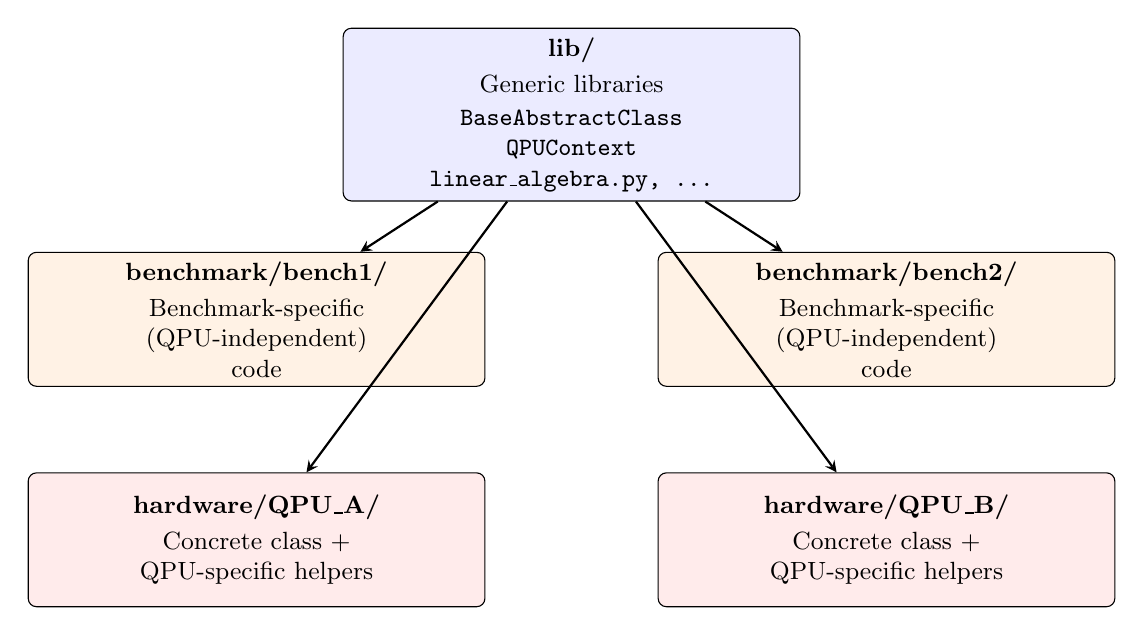
\begin{tikzpicture}[
  box/.style={
    rectangle, draw, rounded corners=3pt,
    minimum width=5.8cm, minimum height=1.7cm,
    align=center, font=\small
  },
  generic/.style={box, fill=blue!8},
  bench/.style={box, fill=orange!10},
  hw/.style={box, fill=red!8},
  arrow/.style={-stealth, thick},
  %dir/.style={font=\ttfamily\footnotesize}
]
  % Generic layer
  \node[generic] (lib) at (0,4.6)
    {\textbf{lib/}\\[2pt]
     Generic libraries\\[1pt]
     \ttfamily BaseAbstractClass\\
     \ttfamily QPUContext\\
     \ttfamily linear\_algebra.py, \ldots};

  % Benchmark layer
  \node[bench] (bench1) at (-4.0,2.0)
    {\textbf{benchmark/bench1/}\\[2pt]
     Benchmark-specific\\
     (QPU-independent)\\
     code};

  \node[bench] (bench2) at (4.0,2.0)
    {\textbf{benchmark/bench2/}\\[2pt]
     Benchmark-specific\\
     (QPU-independent)\\
     code};

  % Hardware / QPU layer
  \node[hw] (qpu1) at (-4.0,-0.8)
    {\textbf{hardware/QPU\_A/}\\[2pt]
     Concrete class +\\
     QPU-specific helpers};

  \node[hw] (qpu2) at (4.0,-0.8)
    {\textbf{hardware/QPU\_B/}\\[2pt]
     Concrete class +\\
     QPU-specific helpers};

  % Arrows
  \draw[arrow] (lib) -- (bench1);
  \draw[arrow] (lib) -- (bench2);
  \draw[arrow] (lib) -- (qpu1);
  \draw[arrow] (lib) -- (qpu2);
\end{tikzpicture}
\end{center}

\begin{itemize}
  \item All algorithmic logic that does not depend on any particular QPU  
        or benchmark belongs in the \texttt{lib/} directory.
  \item Code that is specific to a benchmark but remains independent of the  
        underlying hardware resides under the corresponding  
        \texttt{benchmark/<name>/} subdirectory. 
        It is worth noting that there must be a QPU independent implementation of the benchmark that provides the computation to perform and the computation of the score.
  \item Only the code that realises a concrete QPU (including the three  
        entries of \texttt{capabilitySet}) or that talks directly to a given  
        QPU hardware target lives under the corresponding  
        \texttt{hardware/QPUX/} subdirectory.
        These are the only files that are allowed to import QPU specific libraries (e.g. Qiskit, Ocean, \emph{etc.})
\end{itemize}

This strict separation maximises code reuse, keeps the generic framework stable,  
and makes the addition of a new application or a new QPU a local and  
well-contained change.
\section{Summary}

The combination of

\begin{itemize}
  \item an abstract base class defining a uniform contract,
  \item a \texttt{capabilitySet} dictionary that always contains exactly three function pointers  
        (\texttt{preprocess}, \texttt{run}, \texttt{postprocess}),
  \item a dedicated context object for data exchange, and
  \item a rigid four-step life-cycle  
        (\texttt{\_\_init\_\_} $\to$ preprocess $\to$ run $\to$ postprocess)
\end{itemize}

gives the whole software a clean, extensible and easily maintainable architecture.  Adding a new QPU reduces to writing one new concrete class that implements the abstract methods and registers the three capabilities; the rest of the framework remains untouched.

\section{Short How-to: building a new support for a QPU}

The following describe with more details than in section \ref{sec:concreteQPU} the steps required to implement a new hardware/QPU support.

The global scheme of execution and the philosophy of implementation can be found on figure \ref{fig:arch_3layers_decoupled}.

\begin{figure}[htbp]
\centering
\resizebox{\textwidth}{!}{%
\begin{tikzpicture}[
    node distance=1.1cm and 2.5cm,
    font=\sffamily\small,
    % Layer boxes
    layer/.style={draw=blue!60!black, fill=blue!5, thick, rectangle, rounded corners=6pt, inner sep=12pt},
    layer title/.style={font=\sffamily\bfseries\color{blue!80!black}, anchor=north west},
    % Component nodes
    class node/.style={draw=teal!80!black, fill=teal!10, thick, rectangle, rounded corners=4pt, align=center, minimum width=3.8cm, minimum height=0.9cm},
    func node/.style={draw=orange!80!black, fill=orange!10, thick, rectangle, rounded corners=4pt, align=center, minimum width=3.8cm, minimum height=0.9cm},
    bench node/.style={draw=purple!80!black, fill=purple!10, thick, rectangle, rounded corners=4pt, align=center, minimum width=3.8cm, minimum height=0.9cm},
    % Flow arrows
    call arrow/.style={-{Stealth[scale=1.0]}, thick, color=blue!70!black},
    data arrow/.style={-{Stealth[scale=1.0]}, thick, dashed, color=purple!80!black},
    dict arrow/.style={-{Stealth[scale=1.0]}, thick, dotted, color=teal!80!black}
]

    % ==========================================
    % LAYER 1 (TOP LEFT): FRONT-END / RUNNER
    % ==========================================
    \node[class node] (runner) {\textbf{Front-End / General Runner}\\ \footnotesize\textit{Controls iteration loop \& execution flow}};

    % ==========================================
    % LAYER 2 (TOP RIGHT): BENCHMARK LAYER
    % ==========================================
    \node[bench node, right=3.5cm of runner] (bench_module) {\textbf{Benchmark Score Module}\\ \footnotesize\textit{Extensible: Problem Defs \& Scoring}};

    % ==========================================
    % LAYER 3 (BOTTOM CENTER): HARDWARE BACK-END
    % ==========================================
    % Context and Dictionary (Left side of Back-End)
    \node[class node, below left=2.5cm and -0.5cm of runner] (backend_class) {\textbf{QPUContext}\\ \footnotesize\textit{State Management \& Config}};
    \node[class node, below=0.6cm of backend_class] (dict) {\textbf{Hardware Dictionary}\\ \footnotesize\textit{Function Pointers Lookup}};

    % Free functions (Right side of Back-End, directly under Benchmark Module)
    \node[func node, below=2.5cm of bench_module] (preprocess) {\texttt{preprocess\_benchmark()}\\ \footnotesize\textit{Setup reg/pgm + Fetch problem def}};
    \node[func node, below=0.5cm of preprocess] (run) {\texttt{run\_benchmark()}\\ \footnotesize\textit{Execute on target hardware}};
    \node[func node, below=0.5cm of run] (postprocess) {\texttt{postprocess\_benchmark()}\\ \footnotesize\textit{Format samples $\rightarrow$ ctx.formattedSamples}};

    % ==========================================
    % CONTAINERS / LAYERS (BACKGROUND FIT)
    % ==========================================
    \begin{scope}[on background layer]
        % Layer 1 Box (Front-End)
        \node[layer, fit=(runner), inner sep=12pt] (l1) {};
        \node[layer title] at (l1.north west) {Layer 1: Front-End};

        % Layer 2 Box (Benchmark Support)
        \node[layer, fit=(bench_module), inner sep=12pt] (l2) {};
        \node[layer title] at (l2.north west) {Layer 2: Benchmark Support};

        % Layer 3 Box (Hardware Back-End)
        \node[layer, fit=(backend_class)(dict)(preprocess)(postprocess), inner sep=12pt] (l3) {};
        \node[layer title] at (l3.north west) {Layer 3: Hardware Back-End};
        
        % Sub-group visual separator inside Layer 3
        \node[draw=orange!50, fill=orange!5, dashed, rounded corners=4pt, fit=(preprocess)(run)(postprocess), label={[font=\scriptsize\bfseries\color{orange!80!black}]above:HW-Specific Function Pointers}] (free_funcs_box) {};
    \end{scope}

    % ==========================================
    % CONTROL & DATA FLOWS
    % ==========================================
    % 1. Front-End requests function pointers from Hardware Dictionary
    \draw[call arrow] (runner.south) -- node[left, font=\scriptsize, align=right] {1. Request function pointers\\for target HW} (backend_class.north);
    
    % 2. Dictionary binds function pointers
    \draw[dict arrow] (backend_class) -- (dict);
    \draw[dict arrow] (dict.east) -- node[below, font=\scriptsize] {2. Bind pointers} (free_funcs_box.south west);

    % 3. Preprocess fetches generic problem definition from Benchmark Module
    \draw[data arrow] (bench_module.south) -- node[left, font=\scriptsize] {Problem Def} (preprocess.north);

    % 4. Front-End executes pipeline (Preprocess -> Run -> Postprocess)
    \draw[call arrow] (runner.south east) -- node[above, sloped, font=\scriptsize] {3. Execute loop} (preprocess.north west);
    \draw[call arrow] (preprocess) -- (run);
    \draw[call arrow] (run) -- (postprocess);

    % Context passing (Dashed)
    \draw[data arrow] (backend_class) -- node[above, font=\scriptsize] {\texttt{ctx}} (preprocess);
    \draw[data arrow] (backend_class) -- node[above, font=\scriptsize] {\texttt{ctx}} (run);
    \draw[data arrow] (backend_class) -- node[above, font=\scriptsize] {\texttt{ctx}} (postprocess);

    % 5. Postprocess sends formatted results up to Benchmark Module
    \draw[data arrow] (postprocess.east) .. controls +(right:1.2cm) and +(right:1.2cm) .. 
        node[right, font=\scriptsize, align=left] {4. \texttt{ctx.formattedSamples}} 
        (bench_module.east);

    % 6. Benchmark Module returns status (boolean) and score to Front-End
    \draw[call arrow] (bench_module.west) -- node[above, font=\scriptsize] {5. Boolean \& Score} (runner.east);

\end{tikzpicture}%
}
\caption{Three-layer decoupled architecture: The Front-End orchestrates execution, the pluggable Benchmark Layer defines problem sets and scoring, and the Hardware Back-End handles hardware-specific execution via dynamic function pointers.}
\label{fig:arch_3layers_decoupled}
\end{figure}

\subsection{Header}

Adding support for a new hardware architecture requires creating a dedicated subdirectory inside \texttt{hardware/}. Best practice is to name this directory after the hardware architecture, keeping future variations and upgrades in mind.

Currently, the \texttt{hardware/} directory uses a flat structure. However, as support for more architectures grows, we may introduce an intermediate layer grouped by computing paradigm--such as Gate-based (e.g., supraconducting, trapped ions, optical, etc.) or Quantum Simulators/``analog'' (e.g., quantum annealers, neutral atoms, etc.).

For now, we will stick to the flat structure and simply create a single new subdirectory under hardware/. To set it up:

\begin{itemize}
\item Create a subdirectory named after the new hardware family.
\item Add an \texttt{\_\_init\_\_.py} file (even if empty) so Python recognizes it as a package.
\item Create at least one Python module to implement support for the architecture.
\end{itemize}

The following section outlines the key features and principles required to build a minimal Python support file.

\begin{lstlisting}[language=Python, caption={Example of Python header for a QPU module}]
import numpy as np
import [other generic support libraries for your code]
# add project root to python path
from pathlib import Path
root = Path(__file__).resolve().parents[2]   
sys.path.insert(0, str(root))
# then we can import libraries from project
from lib.QPUBenchClass import *
from lib.linear_algebra_ising import *
# last but not least: import the relevant python libraries for the new QPU 
import ... # e.g. qiskit, dimod, myqlm, etc.
\end{lstlisting}

\subsection{Backend functions}

Next, you need to implement the core support functions. For each benchmark score, the module must provide the following three functions:

\begin{itemize}
    \item \texttt{preprocess\_benchmark}: Sets up the hardware registers and prepares the program to run the benchmark. Crucially, this function must utilize the generic problem definitions provided by the corresponding benchmark score modules.
    \item \texttt{run\_benchmark}: Executes the benchmark. While execution logic is often generic across benchmarks on a given QPU, specific hardware constraints may require custom behavior.
    \item \texttt{postprocess\_benchmark}: Processes and formats the QPU-specific samples collected in \texttt{QPUContext} during execution. It returns two items:
    \begin{enumerate}
        \item A ternary flag indicating execution status (\texttt{True} to continue iterating, \texttt{False/0} when iterations are complete and the score can be computed). The ternary value (-1) is used if the iteration is required to continue without incrementing the counter value.
        \item A normalized sample format ready for processing by the generic benchmark score implementation.
    \end{enumerate}
\end{itemize}

All three functions share state primarily via the QPU context, receiving an \texttt{QPUContext} object as a parameter.

Naturally, developpers are free to implement any support function support they need to for a sound software design.

\subsection{Concrete class implementation}

Lastly, the module must provide a concrete class instanciation of the generic QPUBenchClass from whom it must inherit.

The important parts for data are:
\begin{itemize}
	\item \texttt{capabilitySet}: provides the list of the benchmark scores supported by the QPU as a list of strings.
	\item \texttt{cpuDispatch}: is the main dictionnary that allows the main program to perform the callback mechanism. Each entry of the dictionnary have its key as the name of the benchmark score, and a list of 3 functions (callback functions) for preprocessing, running an iteration and postprocessing the iteration, as described in the previous section.
\end{itemize}

Regarding the class methods, the important elements to implement are:
\begin{itemize}
	\item The constructor (\texttt{\_\_init\_\_}) that will be called by the main program to start the concrete instanciation. N.B.: the constructor must call the \texttt{selectBenchmark} method (see below).
	\item The \texttt{add\_arguments} that provides the QPU-dependent arguments for the Command Line Interface (CLI) of the main program.
	\item The \texttt{selectBenchmark} method called by the constructor sets the \texttt{preprocessIteration}, \texttt{computeIteration} and \texttt{postprocessIteration} with the pointers to the backend functions that are in the dictionnary. Therefore, a call to any of these 3 methods from the main program will utilize the correct backend function.
	\item The 3 class-backend methods \texttt{preprocessIteration}, \texttt{computeIteration} and \texttt{postprocessIteration} that must called the corresponding backend functions set by the \texttt{selectBenchmark} method.
\end{itemize}

This enables to provide a hardware and benchmark agnostic code execution, where the frontend will call seamlessly the correct and corresponding backend functions.

\subsection{Hardware-Independent Sample Representation}

The \texttt{postprocess\_benchmark} function is responsible for populating the hardware-independent \texttt{ctx.formattedSample} attribute. The generic benchmark module relies on this structure to evaluate whether to stop iterating and to compute the final benchmark score.
The formatted results must be structured as a tuple containing:
\begin{itemize}
	\item The candidate solution vectors.
	\item The number of occurrences for each candidate solution.
	\item the third can be the associated cost/energy.
\end{itemize}
Based on this standardized format, the frontend benchmark function evaluates the stopping condition. Once iterations are complete, it computes the final score for the selected benchmark.

%\appendix
\section*{Appendices}
\setcounter{section}{0}
\renewcommand{\thesection}{\thechapter.\Alph{section}}

% 1. The automatically generated section
%\addtocontents{toc}{\protect\addtolength{\cftsecnumwidth}{7.5em}}
%\renewcommand{\thesection}{Annex \Alph{section}}
\section{BACQ Benchmark}\label{bacq-benchmark}

Implements the framework of the BACQ Benchmark suite in a plateform
independent way. At the moment, it provides supports for the following
QPUs:

\begin{itemize}
\tightlist
\item
  Generic CPU (for reference)
\item
  Dwave
\item
  (TBA) Pasqal (Ruby machine from Genci)
\end{itemize}

And the following scores:

\begin{itemize}
\tightlist
\item
  G-Score (Evaluation of Quantum Optimization heuristics)
\item
  Lin2Score (Evaluation of capability for linear system solving in
  binary)
\end{itemize}

\subsection{📋 Prerequisites}\label{prerequisites}

\begin{itemize}
\tightlist
\item
  Python \textgreater= 3.10
\item
  CMake \textgreater= 3.18
\item
  Compilateur C++ (GCC/Clang)
\item
  Doxygen
\item
  Compilateur Latex (pdflatex)
\item
  Pandoc
\end{itemize}

\subsection{🚀 Installation}\label{installation}

\begin{itemize}
\tightlist
\item
  Build \& install
\end{itemize}

\begin{lstlisting}[language=bash]
git clone [https://github.com/utilisateur/mon-projet.git](https://github.com/utilisateur/mon-projet.git)
cd BacqBench
mkdir build && cd build
cmake ..
make
\end{lstlisting}

\begin{itemize}
\tightlist
\item
  Installation as python package (necessary for use with QPUs)

  \begin{itemize}
  \tightlist
  \item
    inside the main directory ``cd ..'' if required
  \item
    activate your current QPU environement (e.g.~DWave Ocean, Pasqal
    Pulser)
  \item
    install benchmark package using ``pip install -e .''
  \item
    N.B. you can do it after runing the tests (see below) Installing in
    the support environement of your QPU is necessary to run the QPU
    backend of the benchmark suite.
  \end{itemize}
\end{itemize}

\subsection{Basic unitary tests}\label{basic-unitary-tests}

\begin{lstlisting}[language=bash]
make check 
\end{lstlisting}

This provides several unitary tests. Not all are implemented yet.

\subsection{Usage}\label{usage}

The main python script is BACQBenchmark at the root of the project The
minimum parameter is the target QPU (or CPU comparison) E.g.

\begin{lstlisting}[language=bash]
python3 BACQBenchmak dwave 
\end{lstlisting}

Will launch the G-Score evaluation on the default architecture of DWave
(Advantage/Pegasus ATM). It is worth noting that this requires the
BACQBenchmak to be installed as package in the QPU environement. If it
is not the case, the main program would display ``Backend XXX not
available''

E.g.

\begin{lstlisting}[language=bash]
python3 BACQBenchmak cpu 
\end{lstlisting}

To run the G-Score on Simulated Annealing (CPU backend)

Use

\begin{lstlisting}[language=bash]
python3 BACQBenchmak -h
\end{lstlisting}

or

\begin{lstlisting}[language=bash]
python3 BACQBenchmak --help 
\end{lstlisting}

To be provided with usage. Each backend should provide its own help, but
in this case it is necessary to provide the backend on the command line

Being Alpha release, all options may not be implemented yet

\subsection{To do}\label{to-do}

Here is a preliminary of pending functionalities:

\begin{itemize}
\tightlist
\item
  Saving log in json
\item
  Evaluation of benchmark from json results file
\end{itemize}


\section{Doxygen documentation}
% 2. The Doxygen PDF documentation

\includepdf[
  pages=-,                      % include all pages
  pagecommand={\thispagestyle{plain}},  % optional: keep page numbers
  scale=0.95,                   % slightly smaller so margins look good
  offset=0mm 0mm
]{documentation.pdf}    % name of the Doxygen PDF

%\end{appendices}
